\section{Related Work}

\subsection{Infsoft}

Infsoft is a german software company, which specializes in indoor tracking, positioning and navigation. They use custom \emph{infsoft Locator Nodes}\footnote{\url{https://www.infsoft.com/de/technologie/hardware/infsoft-locator-nodes}}, which enable to detect the position of devices trough WiFi or Bluetooth, but can also track the location of RFID chips or utilize Ultra-wideband technology.

This location data is then analyzed to track the path of employees, visitors or objects. These analytics are available in real-time over a web interface, which includes a live rendering of a heatmap, showing locations with heavy or low traffic. But also a history of location data can be displayed. The location data of each device is anonymized and can't reveil information about the owner of the device.

\begin{figure}[!hb]
	\centering
	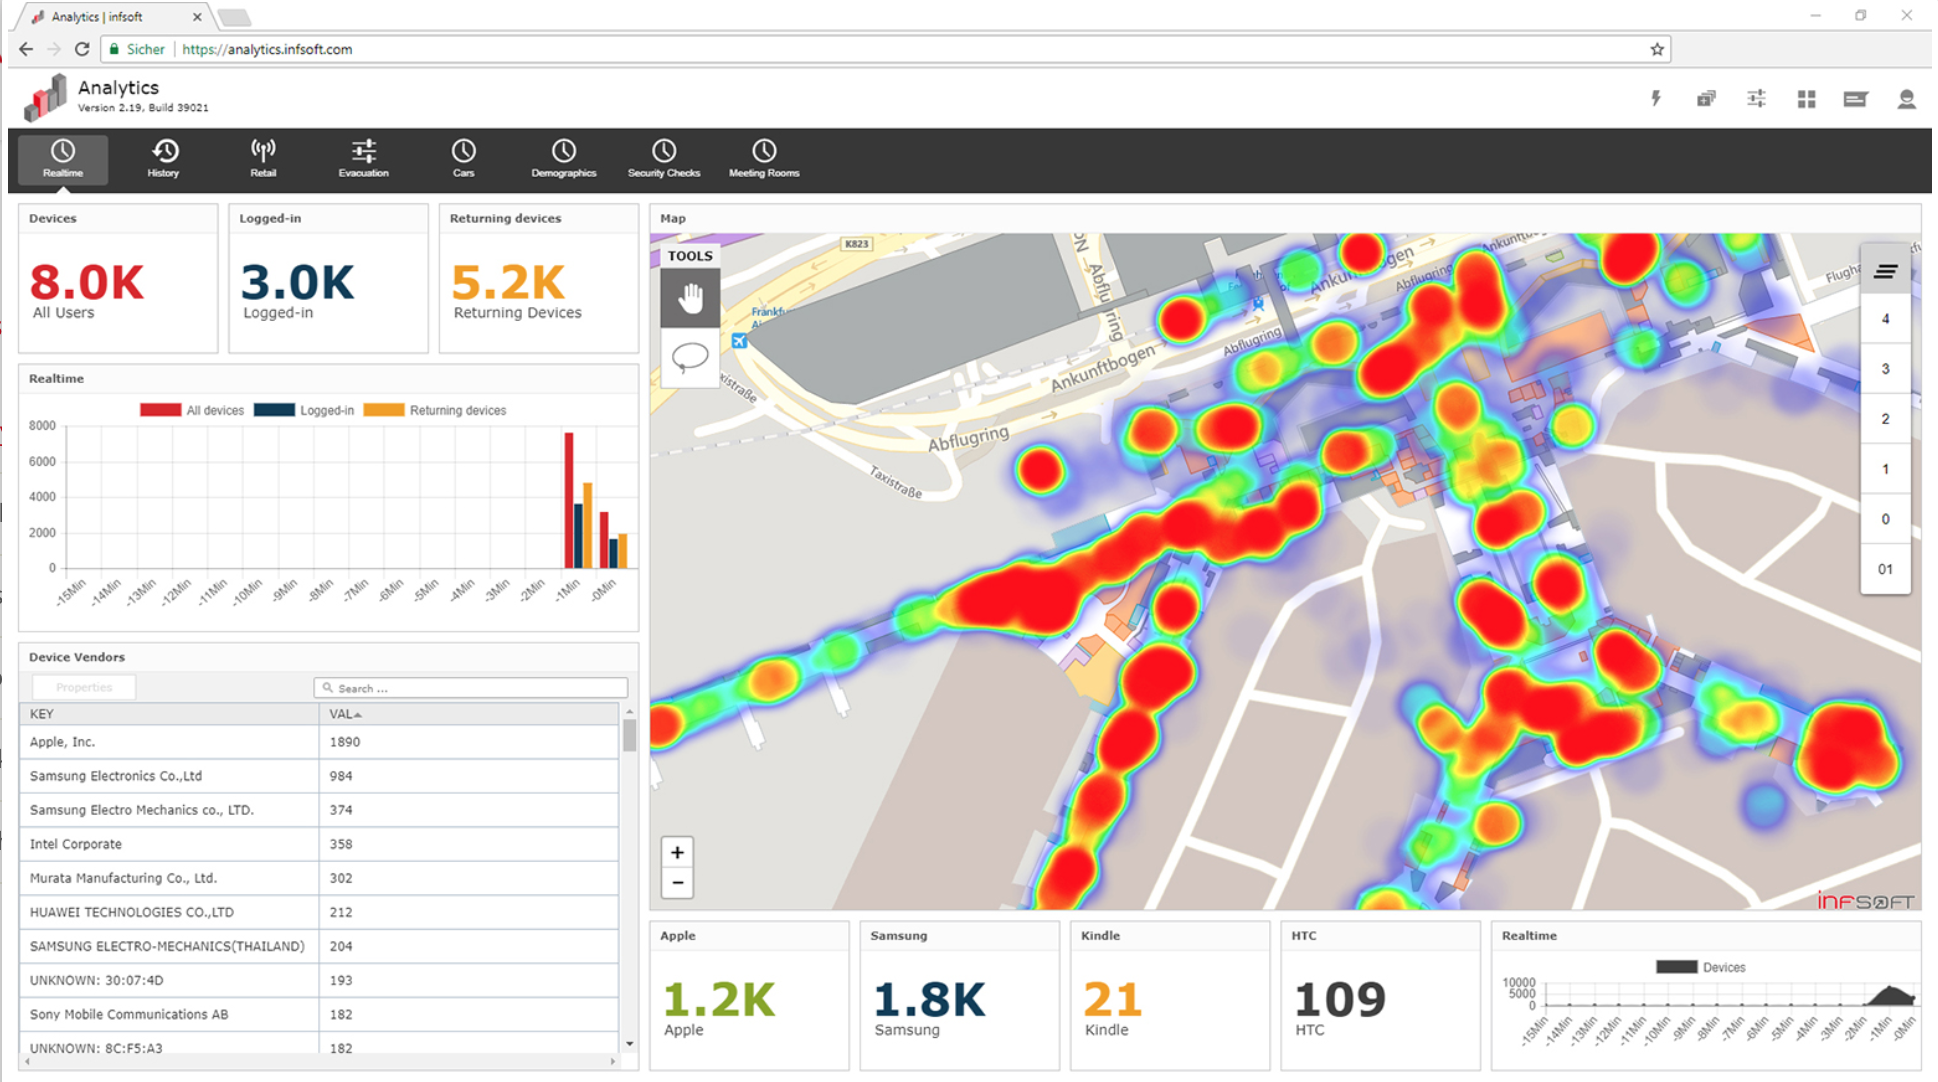
\includegraphics[width=0.9\linewidth]{images/Infsoft}
	\caption{Infsoft Analytics Web Application}
	\label{fig:InfsoftApplication}
\end{figure}

\subsection{Moca}

Moca is a platform for helping companies find out insights about the shopping behavior of their customers. This contains also analytics about the movement paths of the customers in a shopping mall. 
This can be utilized to learn how the customer gets to the retailshop or what they do after leaving the shop.

To achieve this, they use the existing WiFi network setup in the building to track the location of the devices, which has an accuracy of approximately 10 meters\footnote{According to \url{https://www.mocaplatform.com/blog/moca-indoor-location-mobility-flows-for-venues}}. The data is then displayable in a real-time floorplan view with a heatmap overlay. They also allow real-time playbacks of location data from the past days and import of floorplans.

\begin{figure}[!hb]
	\centering
	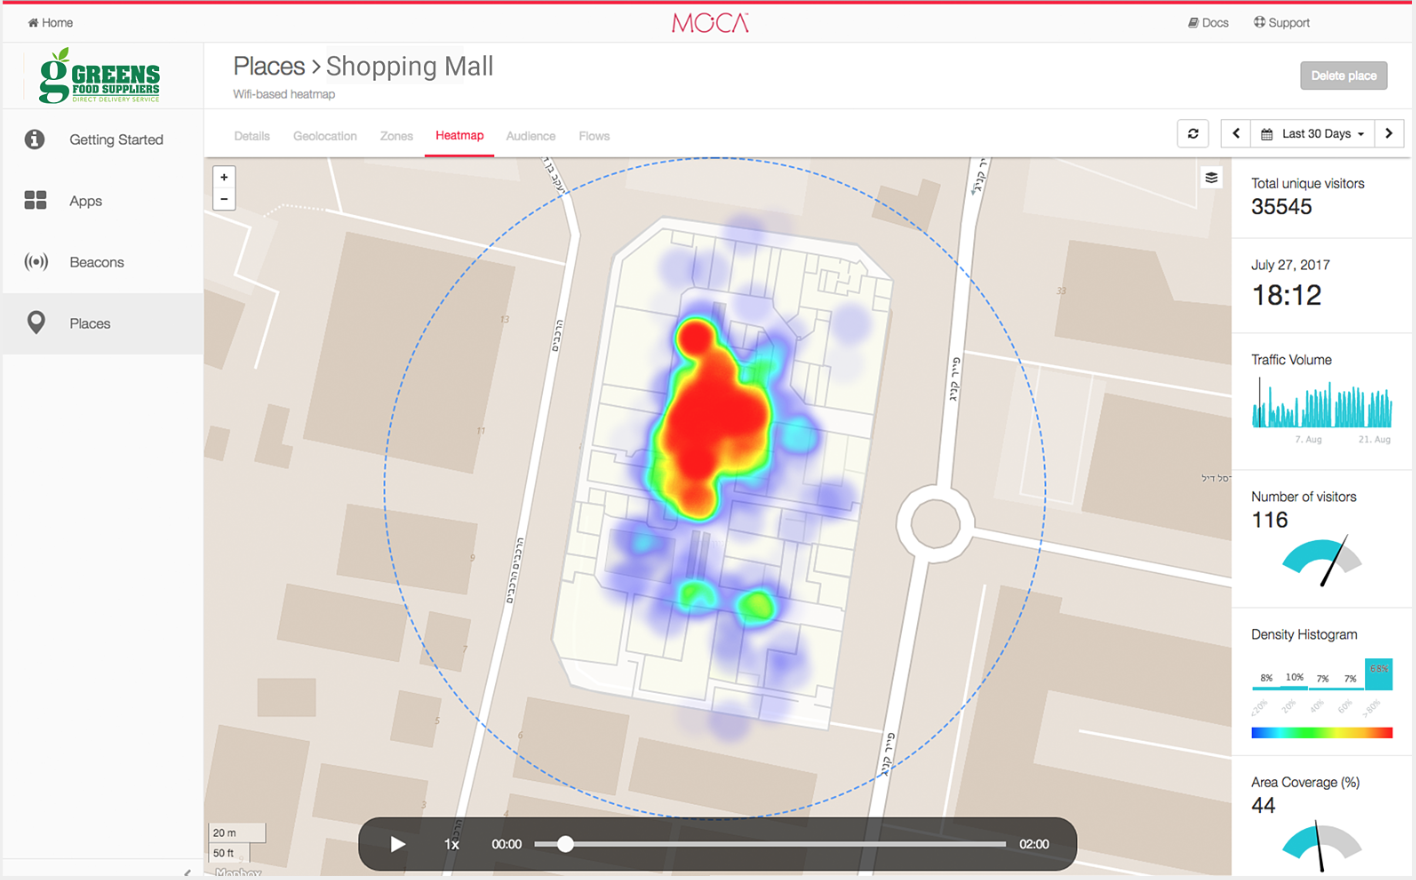
\includegraphics[width=0.9\linewidth]{images/Moca}
	\caption{Moca Web Application}
	\label{fig:InfsoftApplication}
\end{figure}

\clearpage

\subsection{Roommaps}

Roommaps is another indoor information and navigation system, which is primarly focussing on apps for Android and iOS, but is also available as a web application.

The system is also able to track device locations via WiFi signals or Bluetooth beacons and display a heatmap based on this data. 
But unlike the other solutions they support setting detailed data privacy options for each floor. This helps protecting data privacy even more, as it is possible to precisely configure the view access rights for each user for each floor. Additionally, the services are also available for deployment in third party applications.

\subsection{Summary}

All these solutions already offer a great set of functionality. But these are based on the location of devices, which is determined through an indoor positioning sensor network, like a WiFi network or a set of Bluetooth beacons. This makes it unapplicable to our project, because the only data that is available for us are the locations of the gates and the access decisions made at these and not the location of the devices themselves.

Although Roommaps provides their services for third party applications, these services cannot be extended or customized for our use case. 

Additionally, all these services are not open-source products and come with costs regarding hardware and software. Since our project partner requires the use of open-source and free software, the interactive floorplan of our project cannot be based on the related work that was presented and needs to be build from the ground up.

\clearpage